\documentclass[12pt,letterpaper]{article} 
\title{Bangla Spell Checker}
\author{Sanjida samanta\\sanjidasamanta277@gmail.com}
\usepackage{graphicx}
\usepackage{hyperref}
\usepackage{verbatim}
\hypersetup{colorlinks=true,citecolor=blue,linkcolor=black,urlcolor=blue}
\begin{document}
\maketitle
\centering
\vspace{6cm}

\includegraphics[scale=0.5]{bsc.png}
\clearpage
\tableofcontents
\clearpage
\begin{flushleft}
\section{Introduction}
A software application or program feature that identifies Bangla misspelled words and notifies the user,also has it's own keyboard.
Depending on the Bangla spell checker, the feature may automatically show the misspelled word or
provide the user with a list of possible corrections. It gives alternative/correct spellings to the words
you might have confused and misspelled. It scans each and every finds the words in it and compares
each word with a well-known list of spelled words (dictionary). To find out the misspelled Bengali
words use some algorithm like String Matching, Edit Distance which are work of intelligent mixed up.
After implement, then its will be get the most probable suggestion for our misspelled Bengali words. If
a file containing text, is given in this software, one can easily catch the mistakes and can correct them.
For knowing about Bangla spelling, this software is useful.


\section{Target Customers}
\begin{enumerate}
  \item Student 
  \item Teacher 
  \item Journalist who works in Bangla newspaper 
  \item Content Writer 
  \item Government officers 
  \item Who writes document in Bangla 
\end{enumerate}

\section{Features \& Description}
In my proposed software,\\
\textbf{a) File Read and Detection:} The user can input any doc file. If any misspellings are found, then
One window open and show the possible correct word for those misspelled word.\\
\textbf{b) Show Misspelled word:} The words of the file will be checked and misspelled or wrong words
will be marked by red underline.\\
\textbf{c) Correcting Misspelled word with drop down box:} By clicking on the wrong or misspelled
words, as suggestion, a bunch of correct and similar words will be shown.\\
\textbf{d)} If users want, they can add that word to my dictionary.
\section{Algorithm for spell checker}
There are several types of spell checker algorithms. On this thesis described about two
algorithms:\\
\begin{enumerate}
\item \textbf{String Matching}
\item \textbf{Edit Distance}
\item \textbf{Levenshtein distance}
\end{enumerate}
\subsection{String Matching Algorithm}
String matching is an algorithm that attempts to locate one or more strings within a given text. It is an
important class of string algorithms that searches a given position for a single string or multiple strings.\\
\begin{figure}[h]
  \centering
  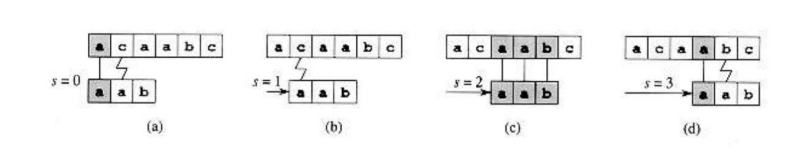
\includegraphics[scale=0.8]{stringmatching.png}
  \caption{Processing on String Matching Algorithm}
  \label{fig:my_picture}
\end{figure}
\subsection{Edit Distance}
Edit distance is a category of such type algorithm which determine the dissimilarity between two or
multiple strings. There are numerous varieties of edit distance. they are –\\
\begin{enumerate}
\item Levenshtein distance
\item Longest common subsequence (LCS)
\end{enumerate}
\subsection{Levenshtein distance}
This distance measures how much minimum operations or single character edits are needed to change 
one string to another. Single character edits mean insertion, substitution or deletion
\begin{figure}[h]
    \centering
    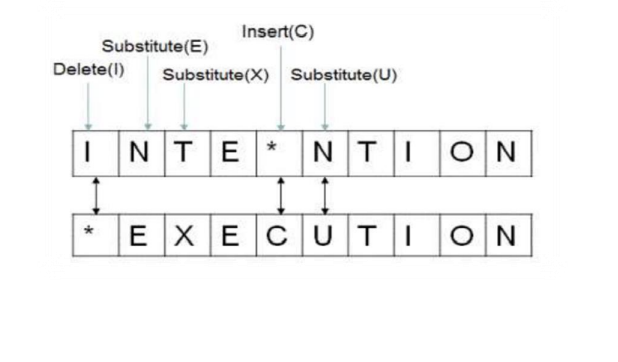
\includegraphics[scale=0.8]{lavestrain.png}
    \caption{ Processing on Levenshtein Distance}
    \label{fig:myfigure}
\end{figure}
\section{User Guide}
\textbf{Step-1:} (Version Guideline)\\
- User must have java 17.0.2 or above version updated on their device.\\
\textbf{Step-2:}
Go to \href{https://download.oracle.com/java/17/archive/jdk-17.0.4.1_windows-x64_bin.msi}{link}. JDK Download for Java download JDK 17.0.2:\\
\begin{enumerate}
\item Accept License Agreement
\item Run the exe for install
\end{enumerate}
\begin{figure}[h]
    \centering
    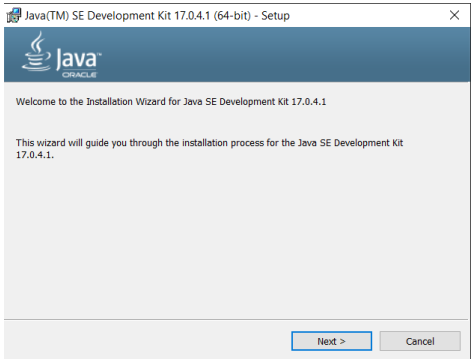
\includegraphics[scale=0.8]{jdk.png}
    \caption{JDK Installation}
    \label{fig:myfigure}
\end{figure}
\textbf{Step-3:}
Once you install Java in windows, click Close
\begin{figure}[h]
    \centering
    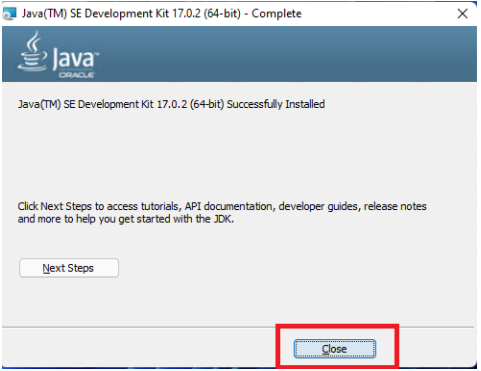
\includegraphics[scale=0.8]{jdkinstall.png}
    \caption{JDK Installation}
    \label{fig:myfigure}
\end{figure} \\
\textbf{Step-4:}
After installing JDK, check with any command prompt to make sure jdk is set in 
device environment
\begin{figure}[h]
    \centering
    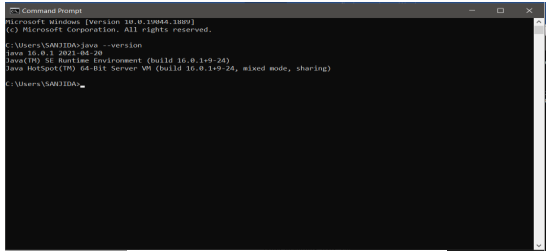
\includegraphics[scale=0.8]{version.png}
    \caption{Java Version Check}
    \label{fig:myfigure}
\end{figure} \\
\textbf{Step-5:}
Then download from here this project.\\
\href{https://github.com/Hima0X2/Bangla_Spell_Checker}{Bangla Spell Checker} \\
\textbf{Step-6:}Then change Text file encoding in 
\begin{verbatim}
UTF_8.
\end{verbatim}
$Properties \to Resource \to Text-file$ encoding in \begin{verbatim}
UTF_8.
\end{verbatim}.
\begin{figure}[h]
    \centering
    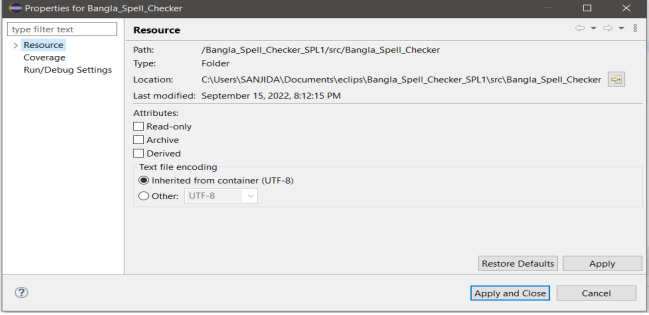
\includegraphics[scale=0.8]{properties.png}
    \caption{Encoding change}
    \label{fig:myfigure}
\end{figure} 
\vspace{0.1cm}
\textbf{Step-7:}After running my code, user will see such kind of Window
\begin{figure}[h]
    \centering
    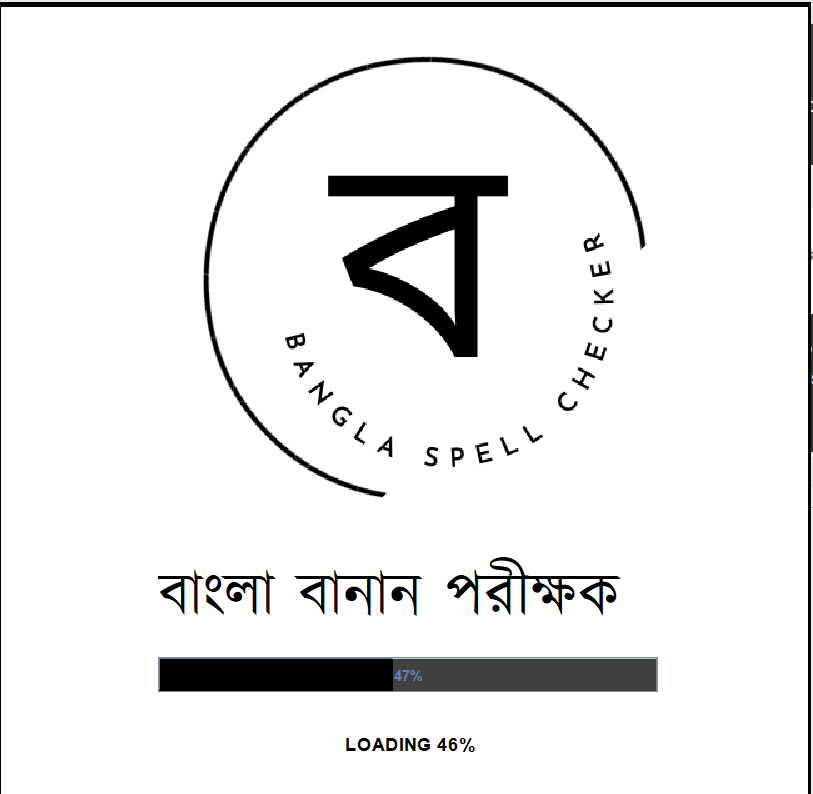
\includegraphics[scale=0.8]{start.png}
    \caption{Starting Window}
    \label{fig:myfigure}
\end{figure} \\
\textbf{Step-8:}
When run the main method, user will see such kind of screen, Then after completing the 
loading Progress bar there will be open the below figure.
\begin{figure}[h]
    \centering
    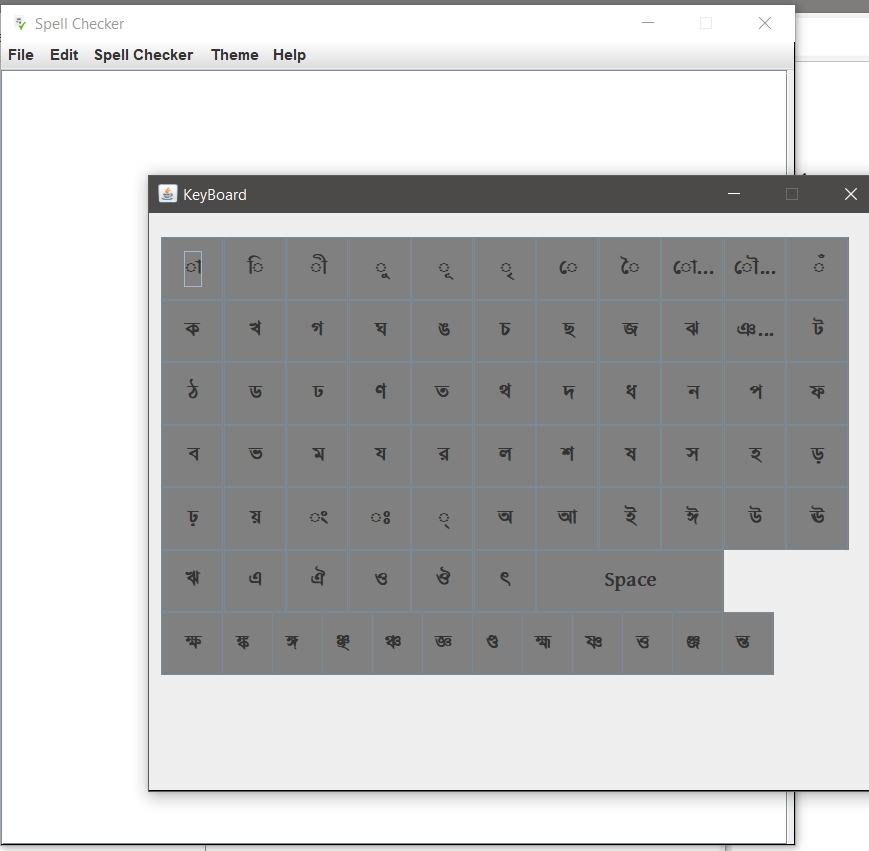
\includegraphics[scale=0.8]{main.png}
    \caption{First Window}
    \label{fig:myfigure}
\end{figure}
In this part,user write some words and click check spell now? If the word is correct then it will remain 
the same.If not then there will be open the below figure

\begin{figure}[h]
    \centering
    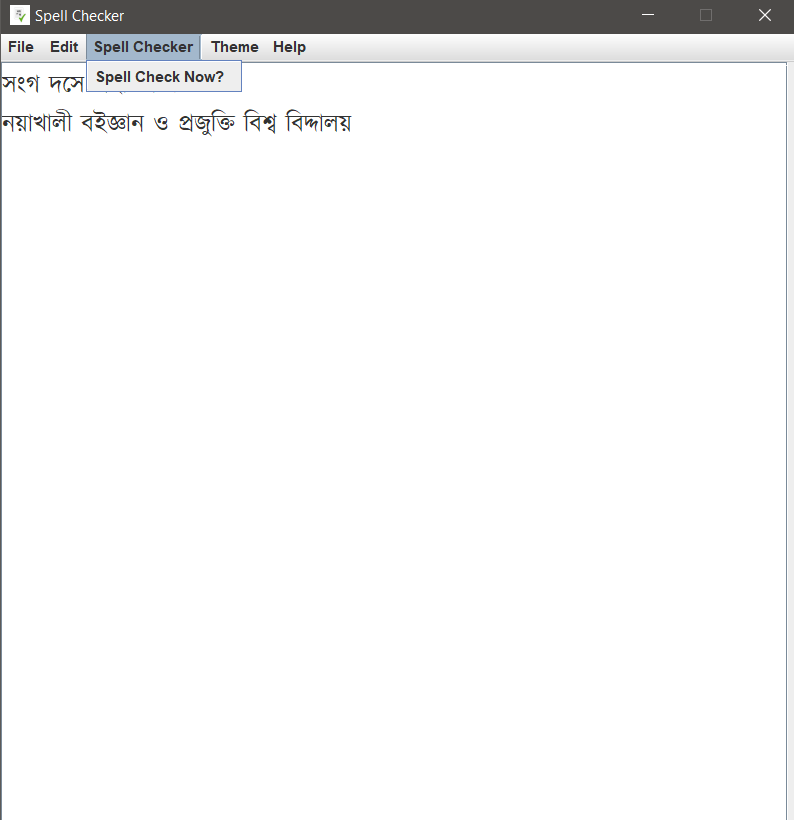
\includegraphics[scale=0.8]{spell.png}
    \caption{Spell Checking Window}
    \label{fig:myfigure}
\end{figure}
Here which word is not found that is show in not found in Dictionary. Here a list of possible words is 
shown in a table. If any word is click then show the Change to textField if change Button is click then 
change the word in spell checking window,if press ignore then ignore this one and if close then close 
the window. \\
\begin{itemize}
  \item[$\cdot$] 
  It also open files
\begin{figure}[htbp]
    \centering
    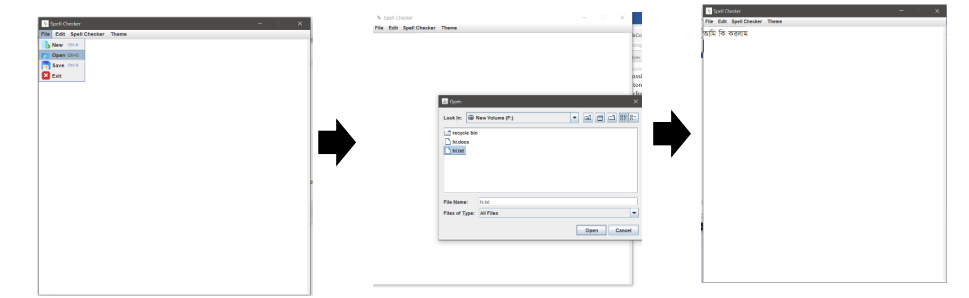
\includegraphics[scale=0.8]{open.png}
    \caption{Open a File from Spell Checking Window}
    \label{fig:myfigure}
\end{figure} \\
  \item[$\cdot$] 
  It also save files
\begin{figure}[htbp]
    \centering
    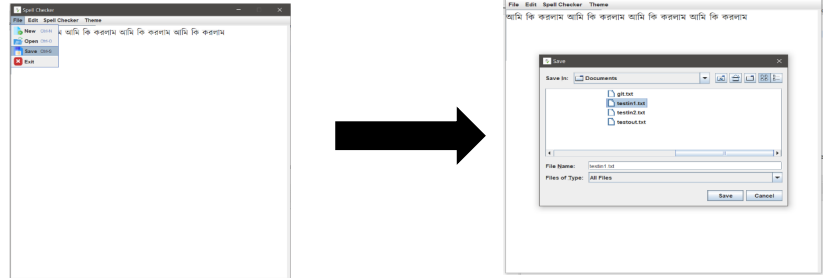
\includegraphics[scale=0.8]{save.png}
    \caption{Save a File to Spell Checking Window}
    \label{fig:myfigure}
\end{figure} \\
  \item[$\cdot$]
  For Exit File
\begin{figure}[htbp]
    \centering
    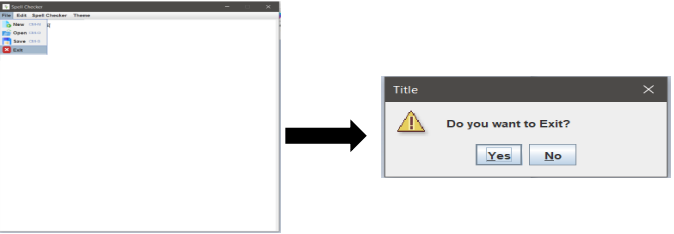
\includegraphics[scale=0.8]{exit.png}
    \caption{Exit File}
    \label{fig:myfigure}
\end{figure} \\
\item[$\cdot$]
For Change Theme
\begin{figure}[htbp]
    \centering
    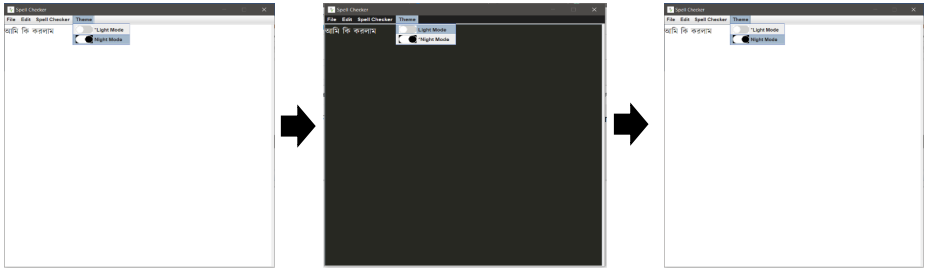
\includegraphics[scale=0.8]{changetheme.png}
    \caption{Theme of Spell Checking Window}
    \label{fig:myfigure}
\end{figure} \\
\end{itemize}
\section{Challenges}
\begin{enumerate}
\item  \textbf{Bangla word:} As unicodes of Bangla words are not well funrnished That’s why it’s a 
hard to handle whose unicodes.
\item  \textbf{Bangla “Juktoborno”:} As I worked with Bangla language, the uniqueness and 
difficulty also in the Bangla is juktoborno.
\item  \textbf{File handling:} As I have restriction of using database, so I have to work with text file. 
And for storing huge amount of words and working with file was a challenge!
\item  \textbf{Algorithm Implementation:} The algorithm I used it could create feature creep problem. 
The feature might not be handy and seems complex to the user.
\item \textbf{Tree and Recursion:} It was hard to create possible words using Tree and Recursion 
for Bangla as Bangla Unicode Doesn’t well funrnished.
\end{enumerate}
\section{Future work}
I will do more with spell checker. I will work with word suggestion and replace 
correct word with wrong word.It will work fine if we write the wrong word of a complex word like 
some Juktoborno and large length of word and using NLP concept.
\section{Conclusion}
In conclusion, while there are currently several options for Bangla spell checkers, there is room for improvement in terms of their accuracy and ability to handle context-dependent spelling errors. By exploring advanced techniques to keep up with changes in the language, it is possible to develop more effective and reliable spell checking tools that meet the needs of Bangla speakers.
\section{Reference}
\textbf{[1]} Introduction to Algorithms by Thomas H. Carmen, Charles E. Leiserson, Ronald L. Rivest, and
Clifford Stein. [Third Edition]\\
\textbf{[2]} Java The Complete Reference by Herbert Scheldt. [ Eleventh Edition]\\
\textbf{[3]} Data Structures by SEYMOUR LIPSCHUTZ [Third Edition]
\end{flushleft}
\end{document}
